The application runs on a single machine, thus making a deployment model non-essential. Data, such as attributes related to stock instances, items, menu items, menus, and orders will be stored in an XML file which will is stored locally on the owner's machine with the added option to import other XML files formed from the same application. The 4-tier system uses a presentation, system, data, and physical layer where each layer interacts only with the layer beneath. This 4-tier system allows an easier transition from using XML files to store data, to using a database management system.
\\ \\
\noindent Originally, the plan was to implement a database into the FoodByte system, though being pressed for time meant that this goal was not achieved. With more time, this 4-tier application allows for simple implementation of a database which would be ideal for larger sets of data though at the moment the FoodByte application just stores data in an XML file called 'data.xml'. The process of saving data checks for corruption by storing data in a 'temp.xml' file then renames this file to 'data.xml'.
\\ \\ 
The system prints customers receipts and chef order slips via the command line interface when orders are finalised. This is because the development team does not yet have the knowledge or hardware to implement physically using the system with a printer to print receipts on command.
\\ \\
\begin{center}
	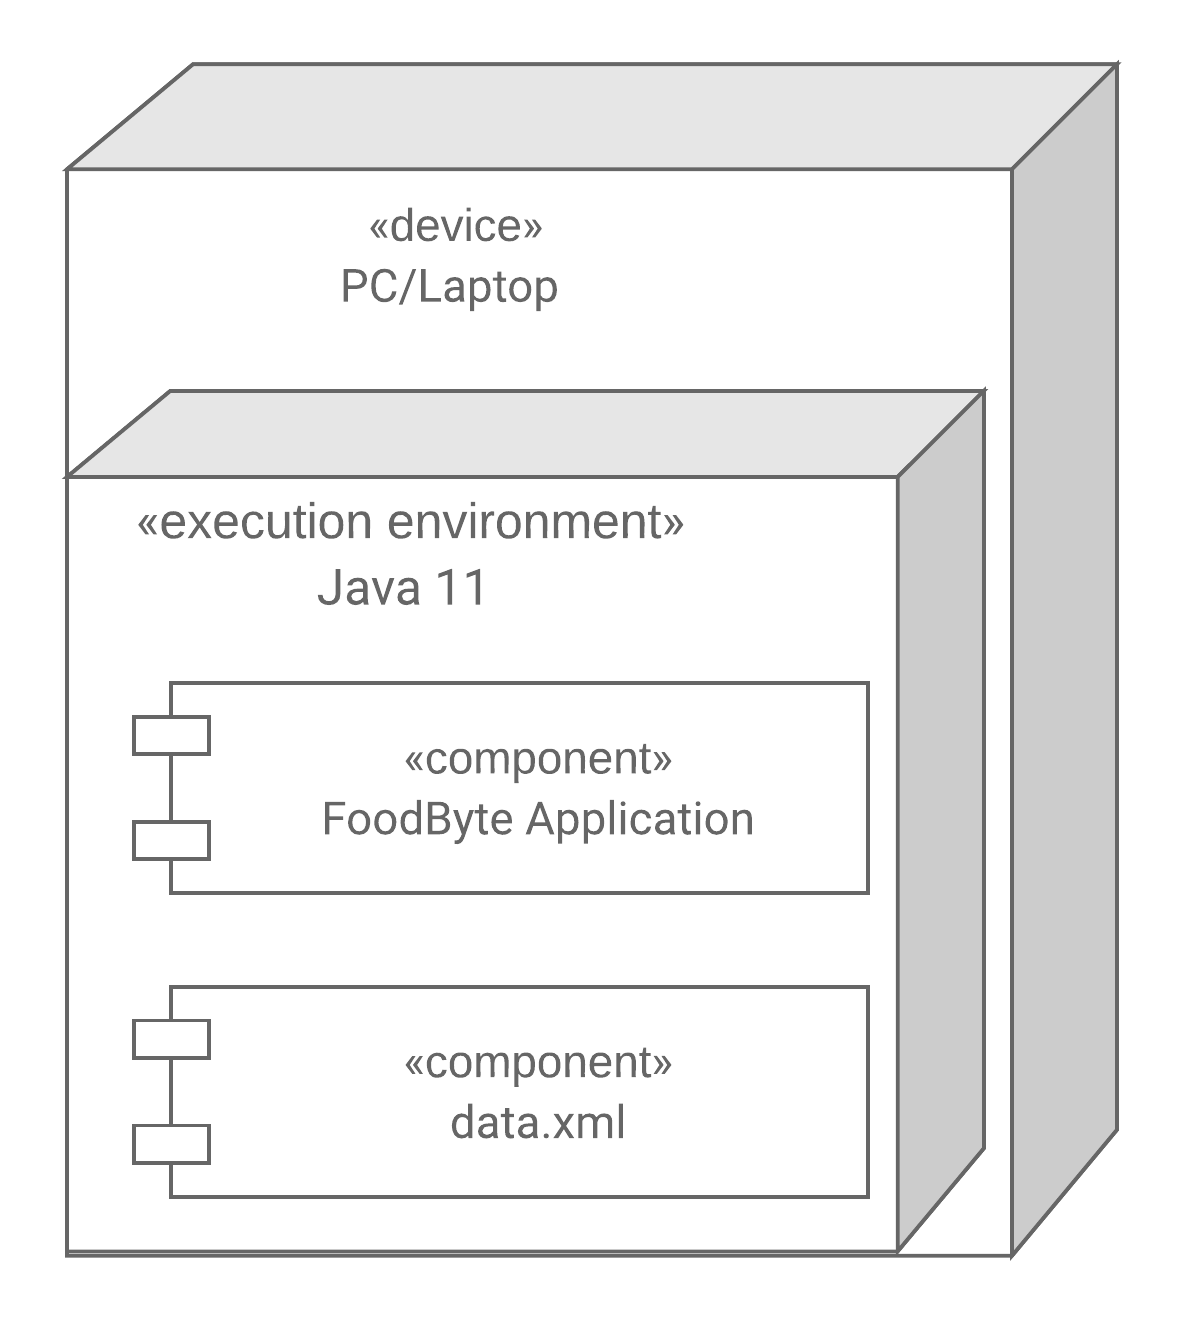
\includegraphics[width=8cm]{images/deployment_diagram.png}
	\\
	Figure 9: UML Deployment Diagram of the system	
\end{center}